\documentclass[title page]{article}
\usepackage{graphicx}
\usepackage{listings}
\usepackage{xcolor}
\usepackage{hyperref}


\title{Automated Video Summarization for Suspicious Event Detection By Making Pipeline}
\author{Syed Muhammad Hussain $\mid$ Azeem Haider $\mid$ Affan Habib}
\date{\today}
\newcommand{\institute}{Habib University}

\begin{document}

\begin{titlepage}
\begin{center}
\vspace*{1cm}
\Large
\textbf{Automated Video Summarization for Suspicious Event Detection By Making Pipeline}

\vspace{0.5cm}
\textbf{\institute}

\vspace{0.5cm}
\textbf{Project Mid Progress Report}

\vspace{1.5cm}
\textbf{Syed Muhammad Hussain $\mid$ Azeem Haider $\mid$ Affan Habib}

\vspace{0.5cm}
\textbf{\today} 
\\ 

\includegraphics[width=10cm]{LOGOHABIB.png} \\

\vfill
\end{center}
\end{titlepage}

\tableofcontents

\newpage

\section{Abstract}

With the widespread use of surveillance cameras in public places, there is an increasing need for automated methods to quickly analyze video footage and detect suspicious events. In this paper, we propose a novel approach for automated video summarization for suspicious event detection by using multi-modal. Our proposed method first extracts visual features from the input video as an event then classifies these events and generates a summary of the events. 
\\ \\
To evaluate the proposed approach, we conduct experiments on a publicly available dataset of surveillance videos. The results demonstrate that our method outperforms existing state-of-the-art techniques in terms of both summarization quality and suspicious event detection accuracy. Our approach can be useful for a variety of real-world applications, such as security surveillance, public safety, and law enforcement.

\section{Introduction}

Surveillance through CCTV cameras has been in the works since the 1940s. Surveillance cameras have proven extremely useful in stopping crime due to the fear of getting caught. However, the sheer amount of data these cameras generate is overwhelming and requires much manual labor to analyze. This is where computer vision comes in. Computer vision is the science of making computers see and understand the world. It is a field that has been proliferating in the past few years. 
\\ \\
With the advent of computer vision technology and algorithms, this manual labor has changed and has been made easier for humanity. Suspicious activity is now tracked through computer vision algorithms that notify the stakeholders when suspicious activity is recognized. Detecting and recognizing suspicious activities to stop them in time is a challenging task. However, with the help of computer vision, this task has become easier by instilling fear in the hearts of the culprits and making catching the culprits easier.
\\ \\
With the crime index of Pakistan being among the highest in the world, especially Karachi standing at 55.0 crime index, suspicious activity detection models have become the need of the hour in the country. Especially completely automated detection models that detect and recognize suspicious activities without human intervention. Summarizing 24-hour CCTV footage is another crucial task for the models to carry out so individuals do not have to skim through the footage to find suspicious activity.
\\ \\
While many models have been proposed in the past, they have yet to be able to achieve the desired results. This is due to various reasons, such as the need for a proper dataset, lack of proper training, and lack of proper testing. In this paper, we propose a novel approach for automated video summarization for suspicious event detection by using multi-modal. Our proposed method first extracts visual features from the input video as an event then classifies these events and generates a summary of the events through the activity labels. We have conducted experiments on a publicly available dataset of surveillance videos. 
\\ \\
Automated security surveillance has become a need of the hour for the people of Pakistan and Karachi. Our model can be a real game changer since it can be used to detect suspicious activities in the city. In addition, the model can also be used to summarize 24-hour CCTV footage so that individuals do not have to skim through entire footage to find suspicious activity.

\section{Dataset}

The DCSASS (Distributed Camera System for Anomaly and Suspicious Spatio-Temporal event detection) dataset available on Kaggle is a video dataset that consists of 3,305 video clips of anomalous and normal events captured by a distributed camera system. This dataset was built based on a dataset created by Sultani et al. (2018) and contains additional annotations and labels.
\\ \\ 
The videos in this dataset were captured at different locations and times, such as airports, train stations, and university campuses. The videos are in the MP4 format and have a resolution of 640x360 pixels. The videos are divided into two classes: normal and anomalous events. The normal events include people walking, standing, and talking, while the anomalous events include actions like fighting, stealing, and vandalism.
\\ \\
This dataset contains videos based on the following 13 classes: Abuse, Arrest, Arson, Assault, Accident, Burglary, Explosion, Fighting, Robbery, Shooting, Stealing, Shoplifting, and Vandalism. Each video is labeled as normal (0) or abnormal (1) according to its content.
\\ \\
The DCSASS dataset includes a subset of surveillance camera videos that contain both normal and anomalous behaviors. Here's a brief overview of this subset:

\begin{itemize}

    \item \textbf{Size} The subset contains a total of 15 videos, each with a duration of approximately 5 minutes.
    \item \textbf{Content} The videos show various scenes, such as arrest, burglary and shooting. The videos contain both normal and anomalous behaviors.
    \item \textbf{Source} The videos were collected from public surveillance cameras in different locations.
    \item \textbf{Usage} The videos can be used for a variety of purposes, such as training and testing of video-based anomaly detection algorithms, research on behavior analysis and crowd detection, and evaluation of surveillance systems.

\end{itemize}
	
The dataset includes annotations for each video clip, including the start and end time of the event, the type of event (normal or anomalous), and a description of the event. Additionally, the dataset includes precomputed optical flow features for each video clip, which can be used for machine learning and computer vision algorithms.
\\ \\
This dataset can be used for research on anomaly detection in surveillance videos and can be used to develop and evaluate algorithms for detecting abnormal events in real-world scenarios.
\\ \\
Overall, the surveillance camera video subset of the DCSASS dataset provides a useful resource for researchers and practitioners in the field of surveillance and security. It provides a realistic and diverse set of videos for testing and evaluation of surveillance systems and anomaly detection algorithms.
\\ \\
All in all, there is a total of 16853 videos, where 9676 videos are labeled as Normal and 7177 as abnormal.

\subsection{Test Dataset}
We will test our model on dataset created and collected by our ownself. Since our project focuses on problems and suspicious activities in the local context, it is imperative to test our model on videos and clips taken in the local surrounding. 
\\ \\
For this purpose, we will be collecting suspicious activity videos from the internet and test our model on them. When collecting data for testing the model, it's important to ensure that the data is diverse and representative of the local context. This can be achieved by collecting videos from various sources, such as social media platforms, local news outlets, and community forums.
\\ \\
To ensure the reliability and authenticity of the data, it's also important to verify the source of each video and confirm that it is not manipulated or altered in any way. This can be done by cross-checking the video with other sources or contacting the original uploader for verification. Furthermore, it's important to consider the privacy and ethical implications of collecting and using this data. To avoid any legal issues or violation of individuals' privacy, the collected videos should be anonymized and any personally identifiable information removed.
\\ \\
Once the data is collected, it's important to label and categorize each video according to the type of suspicious activity captured. This will help in training and testing the model, as well as evaluating its accuracy and effectiveness.
\\ \\
When testing the model, it's important to use a validation dataset to ensure that the model is not overfitting on the training data. This can be done by using a separate dataset for validation and testing purposes, which should also be diverse and representative of the local context.

\section{Methodology}

The objective of this research paper is to present a methodology for efficiently detecting abnormal activity in surveillance videos using a two-stage process. In the first stage, we use OpenCV to summarize long surveillance videos into unique and important events. In the second stage, we use two different approaches, ConvLSTM and LRCN, to detect abnormality in the summarized events based on a training dataset.
\\ \\
The research design consists of the following steps:

\begin{itemize}
    \item \textbf{Data Collection:} The data used in this research was collected from a surveillance system installed in a public area. The data consisted of long surveillance videos of the area.
    \item \textbf{Data Preprocessing:} The collected data was preprocessed to ensure that it was in a suitable format for analysis. This involved converting the video data into frames, which were then analyzed using OpenCV to detect and summarize unique and important events.
    \item \textbf{First Stage Model:} A first-stage model was developed using OpenCV to summarize long surveillance videos into unique and important events. The model uses a combination of image processing techniques, such as background subtraction, object detection, and tracking, to identify important events by frame to frame checking process.
    \item \textbf{Second Stage Models:} Two different models were developed for the second stage: ConvLSTM and LRCN. The ConvLSTM model is a combination of convolutional neural networks and LSTM networks that can learn both spatial and temporal features of the data. The LRCN model is a combination of CNNs and Recurrent Neural Networks (RNNs), specifically Long Short-Term Memory (LSTM) networks, which can effectively capture the temporal dependencies in the data. Both models were trained using a training dataset that included labeled data with normal and abnormal events.
    \item \textbf{Evaluation:} The efficiency and effectiveness of the proposed method will be evaluated using several metrics such as detection rate, false-positive rate, and accuracy. The evaluation will be performed on a separate dataset to ensure the generalizability of the proposed method.   
\end{itemize}

\subsection{Video Summarization Model}

The first stage model is used for motion detection in a video file using the OpenCV library in Python. The model reads a video file and identifies frames where there is a significant change in the content of the video. The method used for motion detection is based on the absolute difference of pixel values between consecutive frames. The code sets a threshold value for the difference between consecutive frames, and if the difference is greater than the threshold, the frame is considered as a unique frame and is written to the output video file. Otherwise, the frame is considered a common frame. The code uses a while loop to read frames from the video until the end of the video is reached. 
\\ \\
The model initialize the counters that are used to keep track of the number of unique frames, common frames, and total frames processed. The output of the model is an output video file that contains only the frames with significant changes in content. The model also prints the total number of frames, the number of unique frames, and the number of common frames detected.

\begin{figure}[h]
    \centering
    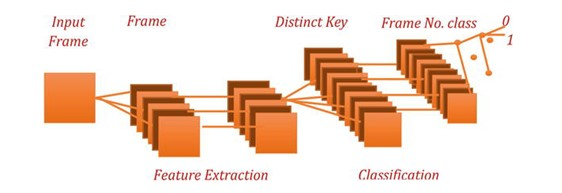
\includegraphics[width=0.6\textwidth]{Picture1.jpg}
    \caption{Image of Memory before Sorting}
    \label{fig:1t}
\end{figure}

We have completed our testing on this model and produced a desired results and pushed this on our Project repository. Here is the link of the first stage model.

\subsection{Abnormal Event Detection Model}

After conducting a thorough literature review, we have selected two approaches for the second stage of our methodology. In this stage, we will analyze and compare both of these approaches for Abnormal Events Detection and Recognition.

\subsubsection{ConvLSTM Approach}

In this step, we implement the first approach by using a combination of ConvLSTM cells. A ConvLSTM cell is a variant of an LSTM network that contains convolutions operations in the network. it is an LSTM with convolution embedded in the architecture, which makes it capable of identifying spatial features of the data while keeping into account the temporal relation. For video classification, this approach effectively captures the spatial relation in the individual frames and the temporal relation across the different frames. As a result of this convolution structure, the ConvLSTM is capable of taking in 3-dimensional input \(width, height, num\_of\_channels\) whereas a simple LSTM only takes in 1-dimensional input hence an LSTM is incompatible for modeling Spatio-temporal data on its own.

\begin{figure}[h]
    \centering
    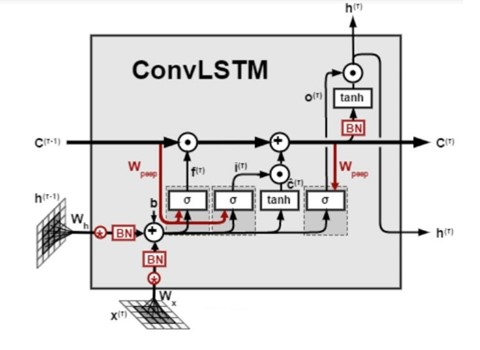
\includegraphics[width=0.6\textwidth]{Picture2.jpg}
    \caption{ConvLSTM Approach}
    \label{fig:2}
\end{figure}

\subsubsection{LRCN Approach}

In this step, we implement the LRCN Approach by combining Convolution and LSTM layers in a single model. Another similar approach can be to use a CNN model and LSTM model trained separately. The CNN model can be used to extract spatial features from the frames in the video, and for this purpose, a pre-trained model can be used, that can be fine-tuned for the problem. And the LSTM model can then use the features extracted by CNN, to predict the action being performed in the video. But here, we implement another approach known as the Long-term Recurrent Convolutional Network (LRCN), which combines CNN and LSTM layers in a single model. 
\\ \\
The Convolutional layers are used for spatial feature extraction from the frames, and the extracted spatial features are fed to LSTM layer\(s\) at each time-steps for temporal sequence modeling. This way the network learns spatiotemporal features directly in an end-to-end training, resulting in a robust model.

\begin{figure}[h]
    \centering
    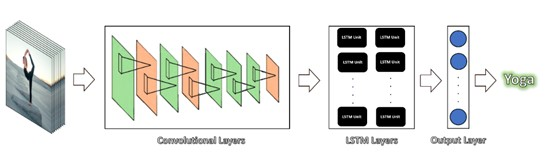
\includegraphics[width=0.6\textwidth]{Picture3.jpg}
    \caption{LRCN Approach}
    \label{fig:3}
\end{figure}

We have completed the preprocessing steps, data set splitting and generation for both approaches. Currently, we are in the process of creating the data set required to train and test these models. here is the link of the model 

\section{Conclusion}

Our project has been carried out in a systematic manner. We first researched about our topic and if it has been covered already. We soon found out that the dual model strategy has not been put into place by anyone yet, and doing that would help people in our city and our country. 
\\ \\
We then moved on to writing a literature review, which we have submitted as our previous submission, at the end of the literature review we had a good enough idea what work has already been carried out and what we can do to differentiate our project from pre-existing work. 
\\ \\
The next stage which we are also done with, is selecting the dataset, as described in the section for Dataset, we will be training our model of the DCSASS dataset and then testing it on dataset we will create ourself from videos collected from the internet.
\\ \\
Finally, we have also researched models for both our purposes. We have finalized the model for video summarization, and have been testing two models the ConvLSTM, and the LRCN model for our object recognition. 
\\ \\
Overall, our project has been moving smoothly and we expect to finish it soon with a high accuracy for our object recognition model. 

\section{Github}

\href{https://github.com/SYED-M-HUSSAIN/Computer-Vision-Research-}{https://github.com/SYED-M-HUSSAIN/Computer-Vision-Research-}

\end{document}
